\documentclass[twoside]{book}

% Packages required by doxygen
\usepackage{calc}
\usepackage{doxygen}
\usepackage{graphicx}
\usepackage[utf8]{inputenc}
\usepackage{makeidx}
\usepackage{multicol}
\usepackage{multirow}
\usepackage{textcomp}
\usepackage[table]{xcolor}

% Font selection
\usepackage[T1]{fontenc}
\usepackage{mathptmx}
\usepackage[scaled=.90]{helvet}
\usepackage{courier}
\usepackage{amssymb}
\usepackage{sectsty}
\renewcommand{\familydefault}{\sfdefault}
\allsectionsfont{%
  \fontseries{bc}\selectfont%
  \color{darkgray}%
}
\renewcommand{\DoxyLabelFont}{%
  \fontseries{bc}\selectfont%
  \color{darkgray}%
}

% Page & text layout
\usepackage{geometry}
\geometry{%
  a4paper,%
  top=2.5cm,%
  bottom=2.5cm,%
  left=2.5cm,%
  right=2.5cm%
}
\tolerance=750
\hfuzz=15pt
\hbadness=750
\setlength{\emergencystretch}{15pt}
\setlength{\parindent}{0cm}
\setlength{\parskip}{0.2cm}
\makeatletter
\renewcommand{\paragraph}{%
  \@startsection{paragraph}{4}{0ex}{-1.0ex}{1.0ex}{%
    \normalfont\normalsize\bfseries\SS@parafont%
  }%
}
\renewcommand{\subparagraph}{%
  \@startsection{subparagraph}{5}{0ex}{-1.0ex}{1.0ex}{%
    \normalfont\normalsize\bfseries\SS@subparafont%
  }%
}
\makeatother

% Headers & footers
\usepackage{fancyhdr}
\pagestyle{fancyplain}
\fancyhead[LE]{\fancyplain{}{\bfseries\thepage}}
\fancyhead[CE]{\fancyplain{}{}}
\fancyhead[RE]{\fancyplain{}{\bfseries\leftmark}}
\fancyhead[LO]{\fancyplain{}{\bfseries\rightmark}}
\fancyhead[CO]{\fancyplain{}{}}
\fancyhead[RO]{\fancyplain{}{\bfseries\thepage}}
\fancyfoot[LE]{\fancyplain{}{}}
\fancyfoot[CE]{\fancyplain{}{}}
\fancyfoot[RE]{\fancyplain{}{\bfseries\scriptsize Generated on Fri Apr 11 2014 11\-:54\-:43 for M\-T\-Fthesisstudies by Doxygen }}
\fancyfoot[LO]{\fancyplain{}{\bfseries\scriptsize Generated on Fri Apr 11 2014 11\-:54\-:43 for M\-T\-Fthesisstudies by Doxygen }}
\fancyfoot[CO]{\fancyplain{}{}}
\fancyfoot[RO]{\fancyplain{}{}}
\renewcommand{\footrulewidth}{0.4pt}
\renewcommand{\chaptermark}[1]{%
  \markboth{#1}{}%
}
\renewcommand{\sectionmark}[1]{%
  \markright{\thesection\ #1}%
}

% Indices & bibliography
\usepackage{natbib}
\usepackage[titles]{tocloft}
\setcounter{tocdepth}{3}
\setcounter{secnumdepth}{5}
\makeindex

% Hyperlinks (required, but should be loaded last)
\usepackage{ifpdf}
\ifpdf
  \usepackage[pdftex,pagebackref=true]{hyperref}
\else
  \usepackage[ps2pdf,pagebackref=true]{hyperref}
\fi
\hypersetup{%
  colorlinks=true,%
  linkcolor=blue,%
  citecolor=blue,%
  unicode%
}

% Custom commands
\newcommand{\clearemptydoublepage}{%
  \newpage{\pagestyle{empty}\cleardoublepage}%
}


%===== C O N T E N T S =====

\begin{document}

% Titlepage & ToC
\hypersetup{pageanchor=false}
\pagenumbering{roman}
\begin{titlepage}
\vspace*{7cm}
\begin{center}%
{\Large M\-T\-Fthesisstudies \\[1ex]\large version0.\-7548743 }\\
\vspace*{1cm}
{\large Generated by Doxygen 1.8.6}\\
\vspace*{0.5cm}
{\small Fri Apr 11 2014 11:54:43}\\
\end{center}
\end{titlepage}
\clearemptydoublepage
\tableofcontents
\clearemptydoublepage
\pagenumbering{arabic}
\hypersetup{pageanchor=true}

%--- Begin generated contents ---
\chapter{Hierarchical Index}
\section{Class Hierarchy}
This inheritance list is sorted roughly, but not completely, alphabetically\-:\begin{DoxyCompactList}
\item \contentsline{section}{Base\-:\-:Database}{\pageref{classBase_1_1Database}}{}
\item \contentsline{section}{Base\-:\-:Data\-Collector}{\pageref{classBase_1_1DataCollector}}{}
\item \contentsline{section}{Base\-:\-:Data\-Output}{\pageref{classBase_1_1DataOutput}}{}
\begin{DoxyCompactList}
\item \contentsline{section}{Base\-:\-:Csv\-Data\-Output}{\pageref{classBase_1_1CsvDataOutput}}{}
\begin{DoxyCompactList}
\item \contentsline{section}{Base\-:\-:Csv\-File\-Data\-Output}{\pageref{classBase_1_1CsvFileDataOutput}}{}
\end{DoxyCompactList}
\item \contentsline{section}{Base\-:\-:File\-Data\-Output}{\pageref{classBase_1_1FileDataOutput}}{}
\begin{DoxyCompactList}
\item \contentsline{section}{Base\-:\-:Csv\-File\-Data\-Output}{\pageref{classBase_1_1CsvFileDataOutput}}{}
\end{DoxyCompactList}
\end{DoxyCompactList}
\item \contentsline{section}{Base\-:\-:Data\-Output\-Builder}{\pageref{classBase_1_1DataOutputBuilder}}{}
\item \contentsline{section}{Base\-:\-:Data\-Provider}{\pageref{classBase_1_1DataProvider}}{}
\item \contentsline{section}{Matrix\-:\-:Matrix\-Builder}{\pageref{classMatrix_1_1MatrixBuilder}}{}
\item \contentsline{section}{Matrix\-:\-:M\-T\-F\-Matrix}{\pageref{classMatrix_1_1MTFMatrix}}{}
\item \contentsline{section}{Tools\-:\-:Processor}{\pageref{classTools_1_1Processor}}{}
\begin{DoxyCompactList}
\item \contentsline{section}{Tools\-:\-:Random\-Tree\-Processor}{\pageref{classTools_1_1RandomTreeProcessor}}{}
\item \contentsline{section}{Tools\-:\-:Tree\-Processor}{\pageref{classTools_1_1TreeProcessor}}{}
\end{DoxyCompactList}
\item \contentsline{section}{Tools\-:\-:Processor\-Factory}{\pageref{classTools_1_1ProcessorFactory}}{}
\item \contentsline{section}{Tree\-:\-:Random\-Tree\-Root}{\pageref{classTree_1_1RandomTreeRoot}}{}
\item \contentsline{section}{Tools\-:\-:Tester}{\pageref{classTools_1_1Tester}}{}
\end{DoxyCompactList}

\chapter{Class Index}
\section{Class List}
Here are the classes, structs, unions and interfaces with brief descriptions\-:\begin{DoxyCompactList}
\item\contentsline{section}{\hyperlink{classBase_1_1CsvDataOutput}{Base\-::\-Csv\-Data\-Output} }{\pageref{classBase_1_1CsvDataOutput}}{}
\item\contentsline{section}{\hyperlink{classBase_1_1CsvFileDataOutput}{Base\-::\-Csv\-File\-Data\-Output} }{\pageref{classBase_1_1CsvFileDataOutput}}{}
\item\contentsline{section}{\hyperlink{classBase_1_1Database}{Base\-::\-Database} }{\pageref{classBase_1_1Database}}{}
\item\contentsline{section}{\hyperlink{classBase_1_1DataCollector}{Base\-::\-Data\-Collector} }{\pageref{classBase_1_1DataCollector}}{}
\item\contentsline{section}{\hyperlink{classBase_1_1DataOutput}{Base\-::\-Data\-Output} }{\pageref{classBase_1_1DataOutput}}{}
\item\contentsline{section}{\hyperlink{classBase_1_1DataOutputBuilder}{Base\-::\-Data\-Output\-Builder} }{\pageref{classBase_1_1DataOutputBuilder}}{}
\item\contentsline{section}{\hyperlink{classBase_1_1DataProvider}{Base\-::\-Data\-Provider} }{\pageref{classBase_1_1DataProvider}}{}
\item\contentsline{section}{\hyperlink{classBase_1_1FileDataOutput}{Base\-::\-File\-Data\-Output} }{\pageref{classBase_1_1FileDataOutput}}{}
\item\contentsline{section}{\hyperlink{classMatrix_1_1MatrixBuilder}{Matrix\-::\-Matrix\-Builder} }{\pageref{classMatrix_1_1MatrixBuilder}}{}
\item\contentsline{section}{\hyperlink{classMatrix_1_1MTFMatrix}{Matrix\-::\-M\-T\-F\-Matrix} }{\pageref{classMatrix_1_1MTFMatrix}}{}
\item\contentsline{section}{\hyperlink{classTools_1_1Processor}{Tools\-::\-Processor} }{\pageref{classTools_1_1Processor}}{}
\item\contentsline{section}{\hyperlink{classTools_1_1ProcessorFactory}{Tools\-::\-Processor\-Factory} }{\pageref{classTools_1_1ProcessorFactory}}{}
\item\contentsline{section}{\hyperlink{classTools_1_1RandomTreeProcessor}{Tools\-::\-Random\-Tree\-Processor} }{\pageref{classTools_1_1RandomTreeProcessor}}{}
\item\contentsline{section}{\hyperlink{classTree_1_1RandomTreeRoot}{Tree\-::\-Random\-Tree\-Root} }{\pageref{classTree_1_1RandomTreeRoot}}{}
\item\contentsline{section}{\hyperlink{classTools_1_1Tester}{Tools\-::\-Tester} }{\pageref{classTools_1_1Tester}}{}
\item\contentsline{section}{\hyperlink{classTools_1_1TreeProcessor}{Tools\-::\-Tree\-Processor} }{\pageref{classTools_1_1TreeProcessor}}{}
\end{DoxyCompactList}

\chapter{Class Documentation}
\hypertarget{classBase_1_1CsvDataOutput}{\section{Base\-:\-:Csv\-Data\-Output Class Reference}
\label{classBase_1_1CsvDataOutput}\index{Base\-::\-Csv\-Data\-Output@{Base\-::\-Csv\-Data\-Output}}
}


{\ttfamily \#include $<$csv\-\_\-data\-\_\-output.\-h$>$}



Inheritance diagram for Base\-:\-:Csv\-Data\-Output\-:\nopagebreak
\begin{figure}[H]
\begin{center}
\leavevmode
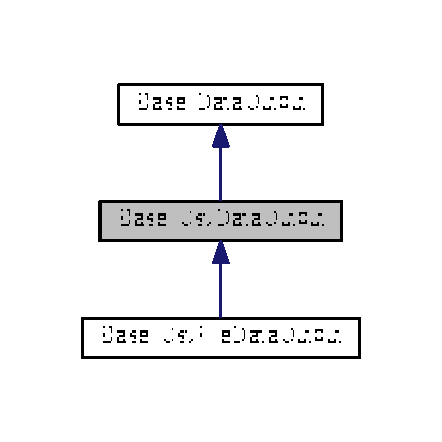
\includegraphics[width=212pt]{classBase_1_1CsvDataOutput__inherit__graph}
\end{center}
\end{figure}


Collaboration diagram for Base\-:\-:Csv\-Data\-Output\-:\nopagebreak
\begin{figure}[H]
\begin{center}
\leavevmode
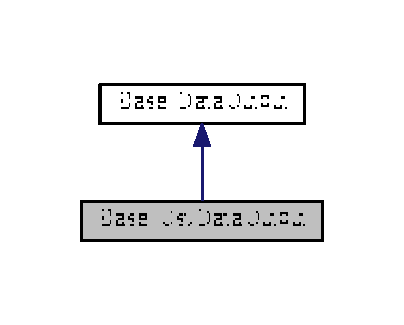
\includegraphics[width=194pt]{classBase_1_1CsvDataOutput__coll__graph}
\end{center}
\end{figure}
\subsection*{Public Member Functions}
\begin{DoxyCompactItemize}
\item 
\hyperlink{classBase_1_1CsvDataOutput_acbedd47083f64caaafc2a33336bef869}{Csv\-Data\-Output} (char separator= '$\vert$')
\item 
virtual \hyperlink{classBase_1_1CsvDataOutput_ac1fbaa916fb293fea40e772397450b5f}{$\sim$\-Csv\-Data\-Output} ()
\item 
virtual void \hyperlink{classBase_1_1CsvDataOutput_a88994527237735d1d6a05cec3b222ba7}{Print\-Line} (int turns\-\_\-count, vector$<$ int $>$ results)
\item 
virtual void \hyperlink{classBase_1_1CsvDataOutput_aa54484865cd138cf49b5aa5b9ef813d5}{Print\-Column\-Titles} ()
\item 
virtual void \hyperlink{classBase_1_1CsvDataOutput_a9302a89524b164d440280bc1c90c90d3}{Set\-Column\-Titles} (vector$<$ string $>$ titles)
\item 
virtual bool \hyperlink{classBase_1_1CsvDataOutput_aaa4e604ce1d06ee002889b2604faf4e4}{Are\-Titles\-Printed} ()
\end{DoxyCompactItemize}
\subsection*{Additional Inherited Members}


\subsection{Detailed Description}
Printer of output in C\-S\-V format. Virtual inheritance used to enable multiple inheritance by child classes \begin{DoxySeeAlso}{See Also}
\hyperlink{classBase_1_1CsvFileDataOutput}{Csv\-File\-Data\-Output} 
\end{DoxySeeAlso}
\begin{DoxyAuthor}{Author}
Jakub Banaszewski 
\end{DoxyAuthor}


\subsection{Constructor \& Destructor Documentation}
\hypertarget{classBase_1_1CsvDataOutput_acbedd47083f64caaafc2a33336bef869}{\index{Base\-::\-Csv\-Data\-Output@{Base\-::\-Csv\-Data\-Output}!Csv\-Data\-Output@{Csv\-Data\-Output}}
\index{Csv\-Data\-Output@{Csv\-Data\-Output}!Base::CsvDataOutput@{Base\-::\-Csv\-Data\-Output}}
\subsubsection[{Csv\-Data\-Output}]{\setlength{\rightskip}{0pt plus 5cm}Base\-::\-Csv\-Data\-Output\-::\-Csv\-Data\-Output (
\begin{DoxyParamCaption}
\item[{char}]{separator = {\ttfamily '$\vert$'}}
\end{DoxyParamCaption}
)}}\label{classBase_1_1CsvDataOutput_acbedd47083f64caaafc2a33336bef869}
Constructor setting default values of class values 
\begin{DoxyParams}{Parameters}
{\em separator} & Char to separate columns of data \\
\hline
\end{DoxyParams}
\hypertarget{classBase_1_1CsvDataOutput_ac1fbaa916fb293fea40e772397450b5f}{\index{Base\-::\-Csv\-Data\-Output@{Base\-::\-Csv\-Data\-Output}!$\sim$\-Csv\-Data\-Output@{$\sim$\-Csv\-Data\-Output}}
\index{$\sim$\-Csv\-Data\-Output@{$\sim$\-Csv\-Data\-Output}!Base::CsvDataOutput@{Base\-::\-Csv\-Data\-Output}}
\subsubsection[{$\sim$\-Csv\-Data\-Output}]{\setlength{\rightskip}{0pt plus 5cm}Base\-::\-Csv\-Data\-Output\-::$\sim$\-Csv\-Data\-Output (
\begin{DoxyParamCaption}
{}
\end{DoxyParamCaption}
)\hspace{0.3cm}{\ttfamily [virtual]}}}\label{classBase_1_1CsvDataOutput_ac1fbaa916fb293fea40e772397450b5f}
Default destructor 

\subsection{Member Function Documentation}
\hypertarget{classBase_1_1CsvDataOutput_aaa4e604ce1d06ee002889b2604faf4e4}{\index{Base\-::\-Csv\-Data\-Output@{Base\-::\-Csv\-Data\-Output}!Are\-Titles\-Printed@{Are\-Titles\-Printed}}
\index{Are\-Titles\-Printed@{Are\-Titles\-Printed}!Base::CsvDataOutput@{Base\-::\-Csv\-Data\-Output}}
\subsubsection[{Are\-Titles\-Printed}]{\setlength{\rightskip}{0pt plus 5cm}virtual bool Base\-::\-Csv\-Data\-Output\-::\-Are\-Titles\-Printed (
\begin{DoxyParamCaption}
{}
\end{DoxyParamCaption}
)\hspace{0.3cm}{\ttfamily [inline]}, {\ttfamily [virtual]}}}\label{classBase_1_1CsvDataOutput_aaa4e604ce1d06ee002889b2604faf4e4}
Getter for are\-\_\-titles\-\_\-printed \begin{DoxyReturn}{Returns}
True if method \hyperlink{classBase_1_1CsvDataOutput_aa54484865cd138cf49b5aa5b9ef813d5}{Print\-Column\-Titles()} was used before, false otherwise 
\end{DoxyReturn}


Implements \hyperlink{classBase_1_1DataOutput_aa201a3a18e148803cc3384af60acda60}{Base\-::\-Data\-Output}.

\hypertarget{classBase_1_1CsvDataOutput_aa54484865cd138cf49b5aa5b9ef813d5}{\index{Base\-::\-Csv\-Data\-Output@{Base\-::\-Csv\-Data\-Output}!Print\-Column\-Titles@{Print\-Column\-Titles}}
\index{Print\-Column\-Titles@{Print\-Column\-Titles}!Base::CsvDataOutput@{Base\-::\-Csv\-Data\-Output}}
\subsubsection[{Print\-Column\-Titles}]{\setlength{\rightskip}{0pt plus 5cm}void Base\-::\-Csv\-Data\-Output\-::\-Print\-Column\-Titles (
\begin{DoxyParamCaption}
{}
\end{DoxyParamCaption}
)\hspace{0.3cm}{\ttfamily [virtual]}}}\label{classBase_1_1CsvDataOutput_aa54484865cd138cf49b5aa5b9ef813d5}
Print titles of columns 

Implements \hyperlink{classBase_1_1DataOutput_a0f1a6127945492d692629120575e7f82}{Base\-::\-Data\-Output}.



Here is the call graph for this function\-:\nopagebreak
\begin{figure}[H]
\begin{center}
\leavevmode
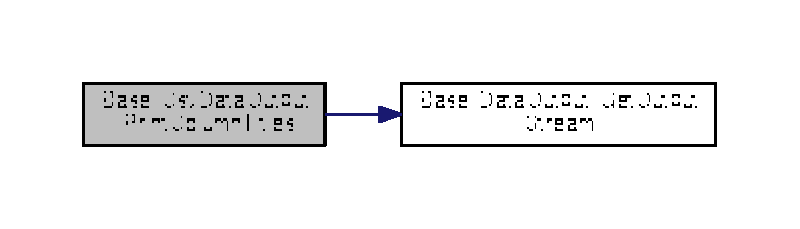
\includegraphics[width=350pt]{classBase_1_1CsvDataOutput_aa54484865cd138cf49b5aa5b9ef813d5_cgraph}
\end{center}
\end{figure}


\hypertarget{classBase_1_1CsvDataOutput_a88994527237735d1d6a05cec3b222ba7}{\index{Base\-::\-Csv\-Data\-Output@{Base\-::\-Csv\-Data\-Output}!Print\-Line@{Print\-Line}}
\index{Print\-Line@{Print\-Line}!Base::CsvDataOutput@{Base\-::\-Csv\-Data\-Output}}
\subsubsection[{Print\-Line}]{\setlength{\rightskip}{0pt plus 5cm}void Base\-::\-Csv\-Data\-Output\-::\-Print\-Line (
\begin{DoxyParamCaption}
\item[{int}]{turns\-\_\-count, }
\item[{vector$<$ int $>$}]{results}
\end{DoxyParamCaption}
)\hspace{0.3cm}{\ttfamily [virtual]}}}\label{classBase_1_1CsvDataOutput_a88994527237735d1d6a05cec3b222ba7}
Print single line of results. 
\begin{DoxyParams}{Parameters}
{\em turns\-\_\-count} & First column of output, number of passed turns(tests) \\
\hline
{\em results} & Vector of \\
\hline
\end{DoxyParams}


Implements \hyperlink{classBase_1_1DataOutput_afdb91464e7559dedf69c56c1b862a216}{Base\-::\-Data\-Output}.



Here is the call graph for this function\-:\nopagebreak
\begin{figure}[H]
\begin{center}
\leavevmode
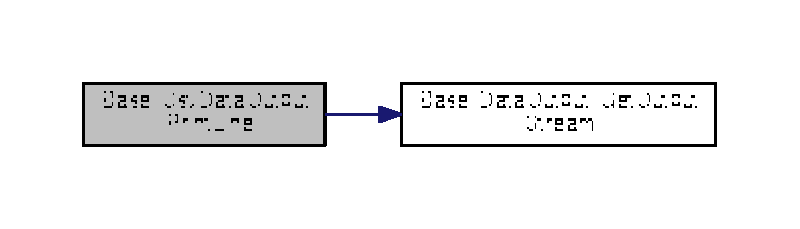
\includegraphics[width=350pt]{classBase_1_1CsvDataOutput_a88994527237735d1d6a05cec3b222ba7_cgraph}
\end{center}
\end{figure}


\hypertarget{classBase_1_1CsvDataOutput_a9302a89524b164d440280bc1c90c90d3}{\index{Base\-::\-Csv\-Data\-Output@{Base\-::\-Csv\-Data\-Output}!Set\-Column\-Titles@{Set\-Column\-Titles}}
\index{Set\-Column\-Titles@{Set\-Column\-Titles}!Base::CsvDataOutput@{Base\-::\-Csv\-Data\-Output}}
\subsubsection[{Set\-Column\-Titles}]{\setlength{\rightskip}{0pt plus 5cm}void Base\-::\-Csv\-Data\-Output\-::\-Set\-Column\-Titles (
\begin{DoxyParamCaption}
\item[{vector$<$ string $>$}]{titles}
\end{DoxyParamCaption}
)\hspace{0.3cm}{\ttfamily [virtual]}}}\label{classBase_1_1CsvDataOutput_a9302a89524b164d440280bc1c90c90d3}
Setter for titles\-\_\-names\-\_\- 
\begin{DoxyParams}{Parameters}
{\em titles} & Titles which replaces titles\-\_\-names\-\_\- \\
\hline
\end{DoxyParams}


Implements \hyperlink{classBase_1_1DataOutput_a368f0c022e828cd3f29085e10e70b113}{Base\-::\-Data\-Output}.



The documentation for this class was generated from the following files\-:\begin{DoxyCompactItemize}
\item 
data\-\_\-managment/csv\-\_\-data\-\_\-output.\-h\item 
data\-\_\-managment/csv\-\_\-data\-\_\-output.\-cpp\end{DoxyCompactItemize}

\hypertarget{classBase_1_1CsvFileDataOutput}{\section{Base\-:\-:Csv\-File\-Data\-Output Class Reference}
\label{classBase_1_1CsvFileDataOutput}\index{Base\-::\-Csv\-File\-Data\-Output@{Base\-::\-Csv\-File\-Data\-Output}}
}


{\ttfamily \#include $<$csv\-\_\-file\-\_\-data\-\_\-output.\-h$>$}



Inheritance diagram for Base\-:\-:Csv\-File\-Data\-Output\-:\nopagebreak
\begin{figure}[H]
\begin{center}
\leavevmode
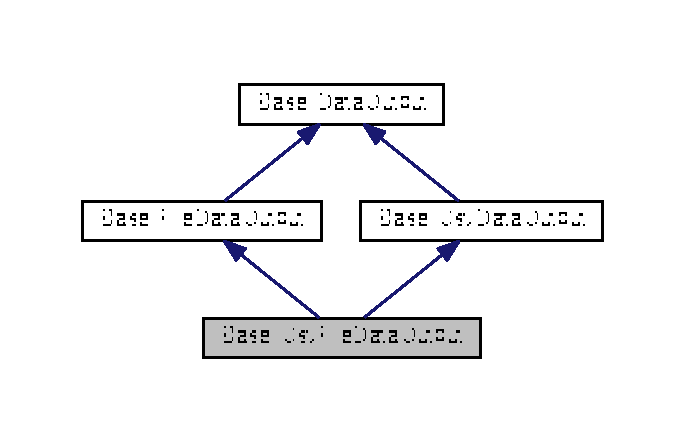
\includegraphics[width=329pt]{classBase_1_1CsvFileDataOutput__inherit__graph}
\end{center}
\end{figure}


Collaboration diagram for Base\-:\-:Csv\-File\-Data\-Output\-:\nopagebreak
\begin{figure}[H]
\begin{center}
\leavevmode
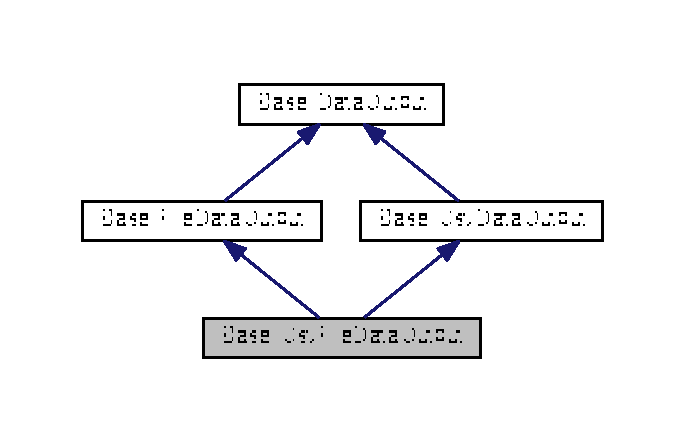
\includegraphics[width=329pt]{classBase_1_1CsvFileDataOutput__coll__graph}
\end{center}
\end{figure}
\subsection*{Public Member Functions}
\begin{DoxyCompactItemize}
\item 
\hyperlink{classBase_1_1CsvFileDataOutput_ac25017da168deaae88ea92dcc5a63611}{Csv\-File\-Data\-Output} (string file\-\_\-path, char separator='$\vert$')
\end{DoxyCompactItemize}
\subsection*{Additional Inherited Members}


\subsection{Detailed Description}
Class to produce output in output file in format C\-S\-V. It has two parent class from which it uses methods. It doesn't have any own method except from contructor. 

\subsection{Constructor \& Destructor Documentation}
\hypertarget{classBase_1_1CsvFileDataOutput_ac25017da168deaae88ea92dcc5a63611}{\index{Base\-::\-Csv\-File\-Data\-Output@{Base\-::\-Csv\-File\-Data\-Output}!Csv\-File\-Data\-Output@{Csv\-File\-Data\-Output}}
\index{Csv\-File\-Data\-Output@{Csv\-File\-Data\-Output}!Base::CsvFileDataOutput@{Base\-::\-Csv\-File\-Data\-Output}}
\subsubsection[{Csv\-File\-Data\-Output}]{\setlength{\rightskip}{0pt plus 5cm}Base\-::\-Csv\-File\-Data\-Output\-::\-Csv\-File\-Data\-Output (
\begin{DoxyParamCaption}
\item[{string}]{file\-\_\-path, }
\item[{char}]{separator = {\ttfamily '$\vert$'}}
\end{DoxyParamCaption}
)}}\label{classBase_1_1CsvFileDataOutput_ac25017da168deaae88ea92dcc5a63611}
Constructor with parameters for parent classes. 
\begin{DoxyParams}{Parameters}
{\em file\-\_\-path} & Needed for \hyperlink{classBase_1_1FileDataOutput}{File\-Data\-Output} \\
\hline
{\em separator} & Needed for \hyperlink{classBase_1_1CsvDataOutput}{Csv\-Data\-Output} \\
\hline
\end{DoxyParams}


The documentation for this class was generated from the following files\-:\begin{DoxyCompactItemize}
\item 
data\-\_\-managment/csv\-\_\-file\-\_\-data\-\_\-output.\-h\item 
data\-\_\-managment/csv\-\_\-file\-\_\-data\-\_\-output.\-cpp\end{DoxyCompactItemize}

\hypertarget{classBase_1_1Database}{\section{Base\-:\-:Database Class Reference}
\label{classBase_1_1Database}\index{Base\-::\-Database@{Base\-::\-Database}}
}


{\ttfamily \#include $<$database.\-h$>$}



\subsection{Detailed Description}
Container of Processor elements. Collect Processors by id or algorithms 

The documentation for this class was generated from the following files\-:\begin{DoxyCompactItemize}
\item 
data\-\_\-managment/database.\-h\item 
data\-\_\-managment/database.\-cpp\end{DoxyCompactItemize}

\hypertarget{classBase_1_1DataCollector}{\section{Base\-:\-:Data\-Collector Class Reference}
\label{classBase_1_1DataCollector}\index{Base\-::\-Data\-Collector@{Base\-::\-Data\-Collector}}
}


{\ttfamily \#include $<$data\-\_\-collector.\-h$>$}

\subsection*{Public Member Functions}
\begin{DoxyCompactItemize}
\item 
\hyperlink{classBase_1_1DataCollector_a3f64da07dd97a418061c7f6e24dd422c}{Data\-Collector} (\hyperlink{classBase_1_1DataProvider}{Data\-Provider} \&data\-\_\-input, shared\-\_\-ptr$<$ \hyperlink{classBase_1_1DataOutput}{Data\-Output} $>$ data\-\_\-output)
\item 
virtual \hyperlink{classBase_1_1DataCollector_aa7deb91a435cbd42091e560e152609ab}{$\sim$\-Data\-Collector} ()
\item 
virtual void \hyperlink{classBase_1_1DataCollector_aa882730336c5d171acfaab053698fe7f}{Add\-Proccessor\-Factory} (shared\-\_\-ptr$<$ \hyperlink{classTools_1_1ProcessorFactory}{Tools\-::\-Processor\-Factory} $>$ procesor\-\_\-factory\-\_\-ptr)
\item 
virtual void \hyperlink{classBase_1_1DataCollector_a5f82cf1aa48981c36cb2e0eba944c148}{Run\-Turns} (int turn\-\_\-amount, bool learn=false)
\item 
virtual void \hyperlink{classBase_1_1DataCollector_afb1d46273c24e3e1fdefba6b730ebf28}{Print\-Actual\-Results} ()
\item 
virtual vector$<$ int $>$ \hyperlink{classBase_1_1DataCollector_afaacb5f36d09faf5e6633a03aa26fdae}{Get\-Result} (int user\-\_\-id)
\item 
virtual vector$<$ int $>$ \hyperlink{classBase_1_1DataCollector_ab300045605fb48a975be8c93f7e93b6f}{Get\-Results\-Sum} ()
\item 
virtual vector$<$ string $>$ \hyperlink{classBase_1_1DataCollector_a52bf3c7c4a610191acd56fa8628ac758}{Get\-Algorithms\-Names} ()
\end{DoxyCompactItemize}


\subsection{Detailed Description}
Class to connect all parts of algorithms. \begin{center}

\begin{DoxyImageNoCaption}
  \mbox{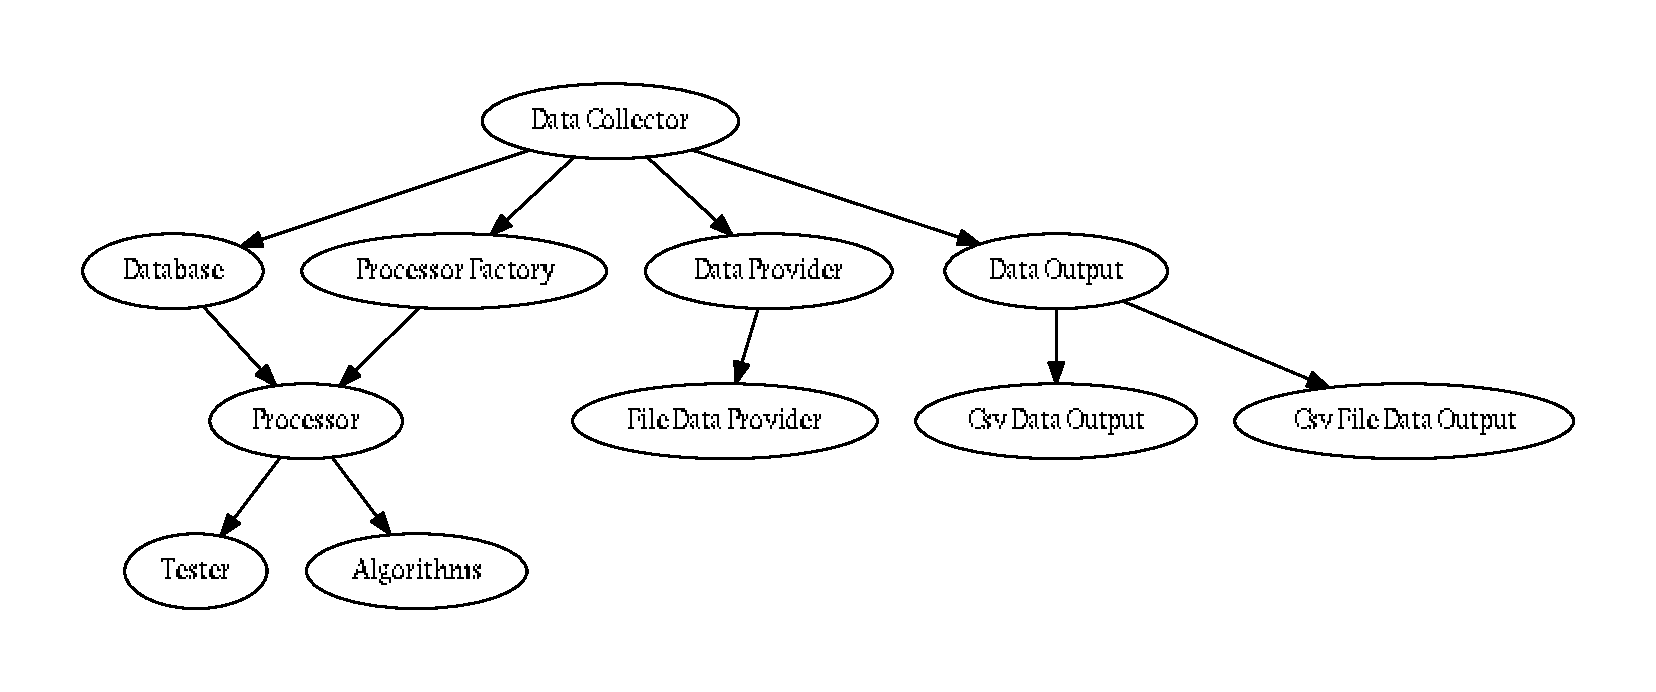
\includegraphics[width=\textwidth,height=\textheight/2,keepaspectratio=true]{dot_inline_dotgraph_1}}
\end{DoxyImageNoCaption}
\end{center}
 It provides data to Processors and print penalties. It also generates Processors for every user, object, contact (id) that comes from \hyperlink{classBase_1_1DataProvider}{Data\-Provider}. \begin{center}

\begin{DoxyImageNoCaption}
  \mbox{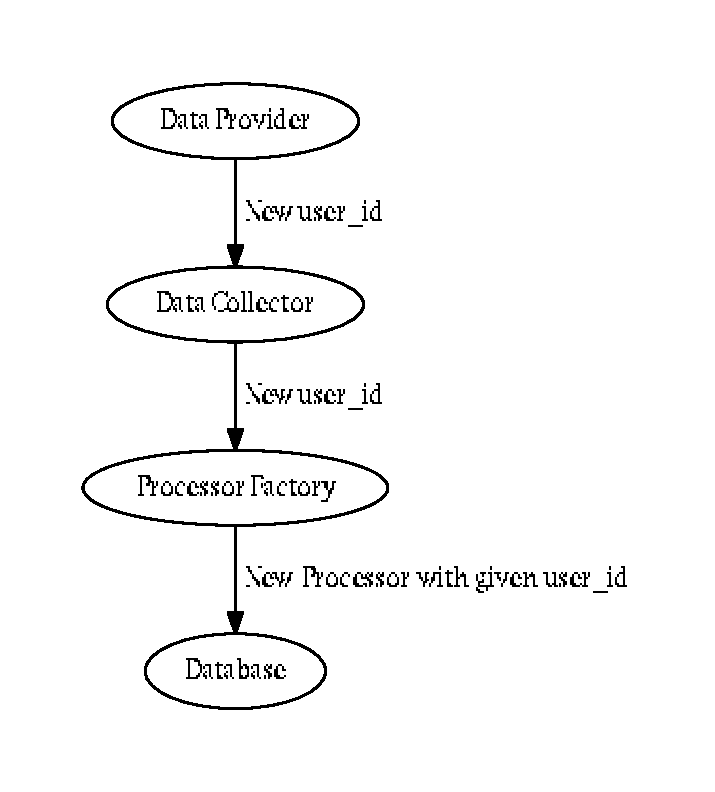
\includegraphics[width=\textwidth,height=\textheight/2,keepaspectratio=true]{dot_inline_dotgraph_2}}
\end{DoxyImageNoCaption}
\end{center}
 Processor\-Factiories are needed to generate Processors for every user (user\-\_\-id) that comes from \hyperlink{classBase_1_1DataProvider}{Data\-Provider}. Every Processor\-Factiory represents one algorithm. 

\subsection{Constructor \& Destructor Documentation}
\hypertarget{classBase_1_1DataCollector_a3f64da07dd97a418061c7f6e24dd422c}{\index{Base\-::\-Data\-Collector@{Base\-::\-Data\-Collector}!Data\-Collector@{Data\-Collector}}
\index{Data\-Collector@{Data\-Collector}!Base::DataCollector@{Base\-::\-Data\-Collector}}
\subsubsection[{Data\-Collector}]{\setlength{\rightskip}{0pt plus 5cm}Base\-::\-Data\-Collector\-::\-Data\-Collector (
\begin{DoxyParamCaption}
\item[{{\bf Data\-Provider} \&}]{data\-\_\-input, }
\item[{shared\-\_\-ptr$<$ {\bf Data\-Output} $>$}]{data\-\_\-output}
\end{DoxyParamCaption}
)}}\label{classBase_1_1DataCollector_a3f64da07dd97a418061c7f6e24dd422c}
Constructor responsible for initialization all connected objects except objects given as parameters 
\begin{DoxyParams}{Parameters}
{\em data\-\_\-input} & Data input to proceed \\
\hline
{\em data\-\_\-output} & Output for results \\
\hline
\end{DoxyParams}
\hypertarget{classBase_1_1DataCollector_aa7deb91a435cbd42091e560e152609ab}{\index{Base\-::\-Data\-Collector@{Base\-::\-Data\-Collector}!$\sim$\-Data\-Collector@{$\sim$\-Data\-Collector}}
\index{$\sim$\-Data\-Collector@{$\sim$\-Data\-Collector}!Base::DataCollector@{Base\-::\-Data\-Collector}}
\subsubsection[{$\sim$\-Data\-Collector}]{\setlength{\rightskip}{0pt plus 5cm}Base\-::\-Data\-Collector\-::$\sim$\-Data\-Collector (
\begin{DoxyParamCaption}
{}
\end{DoxyParamCaption}
)\hspace{0.3cm}{\ttfamily [virtual]}}}\label{classBase_1_1DataCollector_aa7deb91a435cbd42091e560e152609ab}
Default destructor. No object need to be deleted or handled in special way. 

\subsection{Member Function Documentation}
\hypertarget{classBase_1_1DataCollector_aa882730336c5d171acfaab053698fe7f}{\index{Base\-::\-Data\-Collector@{Base\-::\-Data\-Collector}!Add\-Proccessor\-Factory@{Add\-Proccessor\-Factory}}
\index{Add\-Proccessor\-Factory@{Add\-Proccessor\-Factory}!Base::DataCollector@{Base\-::\-Data\-Collector}}
\subsubsection[{Add\-Proccessor\-Factory}]{\setlength{\rightskip}{0pt plus 5cm}void Base\-::\-Data\-Collector\-::\-Add\-Proccessor\-Factory (
\begin{DoxyParamCaption}
\item[{shared\-\_\-ptr$<$ {\bf Tools\-::\-Processor\-Factory} $>$}]{procesor\-\_\-factory\-\_\-ptr}
\end{DoxyParamCaption}
)\hspace{0.3cm}{\ttfamily [virtual]}}}\label{classBase_1_1DataCollector_aa882730336c5d171acfaab053698fe7f}
Method to add Processor\-Factory to generate new Processors \begin{DoxySeeAlso}{See Also}
Processor\-Factory 

Processor 
\end{DoxySeeAlso}

\begin{DoxyParams}{Parameters}
{\em procesor\-\_\-factory\-\_\-ptr} & Pointer to Processor\-Factory which will be added to processor\-\_\-factories\-\_\- vector \\
\hline
\end{DoxyParams}
\hypertarget{classBase_1_1DataCollector_a52bf3c7c4a610191acd56fa8628ac758}{\index{Base\-::\-Data\-Collector@{Base\-::\-Data\-Collector}!Get\-Algorithms\-Names@{Get\-Algorithms\-Names}}
\index{Get\-Algorithms\-Names@{Get\-Algorithms\-Names}!Base::DataCollector@{Base\-::\-Data\-Collector}}
\subsubsection[{Get\-Algorithms\-Names}]{\setlength{\rightskip}{0pt plus 5cm}vector$<$ string $>$ Base\-::\-Data\-Collector\-::\-Get\-Algorithms\-Names (
\begin{DoxyParamCaption}
{}
\end{DoxyParamCaption}
)\hspace{0.3cm}{\ttfamily [virtual]}}}\label{classBase_1_1DataCollector_a52bf3c7c4a610191acd56fa8628ac758}
Method to get names of algorithms put by Processor\-Fatories to processor\-\_\-factories\-\_\- vector; \begin{DoxyReturn}{Returns}
Algorithm names placed in \hyperlink{classBase_1_1DataCollector}{Data\-Collector} 
\end{DoxyReturn}
\hypertarget{classBase_1_1DataCollector_afaacb5f36d09faf5e6633a03aa26fdae}{\index{Base\-::\-Data\-Collector@{Base\-::\-Data\-Collector}!Get\-Result@{Get\-Result}}
\index{Get\-Result@{Get\-Result}!Base::DataCollector@{Base\-::\-Data\-Collector}}
\subsubsection[{Get\-Result}]{\setlength{\rightskip}{0pt plus 5cm}vector$<$ int $>$ Base\-::\-Data\-Collector\-::\-Get\-Result (
\begin{DoxyParamCaption}
\item[{int}]{user\-\_\-id}
\end{DoxyParamCaption}
)\hspace{0.3cm}{\ttfamily [virtual]}}}\label{classBase_1_1DataCollector_afaacb5f36d09faf5e6633a03aa26fdae}
Method to get penalty for one user. Every position on vector represents penalty counted for corresponding algorithm 
\begin{DoxyParams}{Parameters}
{\em user\-\_\-id} & Choosen user \\
\hline
\end{DoxyParams}
\begin{DoxyReturn}{Returns}
Vector of results for given algorithms 
\end{DoxyReturn}
\hypertarget{classBase_1_1DataCollector_ab300045605fb48a975be8c93f7e93b6f}{\index{Base\-::\-Data\-Collector@{Base\-::\-Data\-Collector}!Get\-Results\-Sum@{Get\-Results\-Sum}}
\index{Get\-Results\-Sum@{Get\-Results\-Sum}!Base::DataCollector@{Base\-::\-Data\-Collector}}
\subsubsection[{Get\-Results\-Sum}]{\setlength{\rightskip}{0pt plus 5cm}vector$<$ int $>$ Base\-::\-Data\-Collector\-::\-Get\-Results\-Sum (
\begin{DoxyParamCaption}
{}
\end{DoxyParamCaption}
)\hspace{0.3cm}{\ttfamily [virtual]}}}\label{classBase_1_1DataCollector_ab300045605fb48a975be8c93f7e93b6f}
Method to get penalty sum of every user for every algorithm. Every position on vector represents penalty counted for corresponding algorithm. \begin{DoxyReturn}{Returns}
Vector of sum results for given algorithms 
\end{DoxyReturn}
\hypertarget{classBase_1_1DataCollector_afb1d46273c24e3e1fdefba6b730ebf28}{\index{Base\-::\-Data\-Collector@{Base\-::\-Data\-Collector}!Print\-Actual\-Results@{Print\-Actual\-Results}}
\index{Print\-Actual\-Results@{Print\-Actual\-Results}!Base::DataCollector@{Base\-::\-Data\-Collector}}
\subsubsection[{Print\-Actual\-Results}]{\setlength{\rightskip}{0pt plus 5cm}void Base\-::\-Data\-Collector\-::\-Print\-Actual\-Results (
\begin{DoxyParamCaption}
{}
\end{DoxyParamCaption}
)\hspace{0.3cm}{\ttfamily [virtual]}}}\label{classBase_1_1DataCollector_afb1d46273c24e3e1fdefba6b730ebf28}
Method prints one line of results using \hyperlink{classBase_1_1DataOutput}{Data\-Output} instance \begin{DoxySeeAlso}{See Also}
\hyperlink{classBase_1_1DataOutput}{Data\-Output} 
\end{DoxySeeAlso}


Here is the call graph for this function\-:
\nopagebreak
\begin{figure}[H]
\begin{center}
\leavevmode
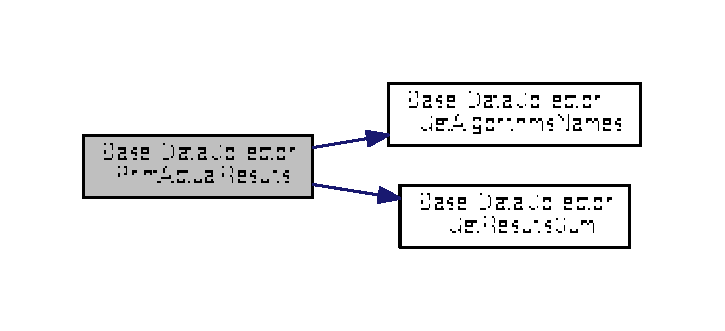
\includegraphics[width=348pt]{classBase_1_1DataCollector_afb1d46273c24e3e1fdefba6b730ebf28_cgraph}
\end{center}
\end{figure}


\hypertarget{classBase_1_1DataCollector_a5f82cf1aa48981c36cb2e0eba944c148}{\index{Base\-::\-Data\-Collector@{Base\-::\-Data\-Collector}!Run\-Turns@{Run\-Turns}}
\index{Run\-Turns@{Run\-Turns}!Base::DataCollector@{Base\-::\-Data\-Collector}}
\subsubsection[{Run\-Turns}]{\setlength{\rightskip}{0pt plus 5cm}void Base\-::\-Data\-Collector\-::\-Run\-Turns (
\begin{DoxyParamCaption}
\item[{int}]{turn\-\_\-amount, }
\item[{bool}]{learn = {\ttfamily false}}
\end{DoxyParamCaption}
)\hspace{0.3cm}{\ttfamily [virtual]}}}\label{classBase_1_1DataCollector_a5f82cf1aa48981c36cb2e0eba944c148}
Method to run Processors. Every turn means one line of input is read and proceed by Processors. 
\begin{DoxyParams}{Parameters}
{\em turn\-\_\-amount} & Number of input line to proceed \\
\hline
{\em learn} & If true then no penalty is added. \\
\hline
\end{DoxyParams}


The documentation for this class was generated from the following files\-:\begin{DoxyCompactItemize}
\item 
data\-\_\-managment/data\-\_\-collector.\-h\item 
data\-\_\-managment/data\-\_\-collector.\-cpp\end{DoxyCompactItemize}

\hypertarget{classBase_1_1DataOutput}{\section{Base\-:\-:Data\-Output Class Reference}
\label{classBase_1_1DataOutput}\index{Base\-::\-Data\-Output@{Base\-::\-Data\-Output}}
}


{\ttfamily \#include $<$data\-\_\-output.\-h$>$}



Inheritance diagram for Base\-:\-:Data\-Output\-:\nopagebreak
\begin{figure}[H]
\begin{center}
\leavevmode
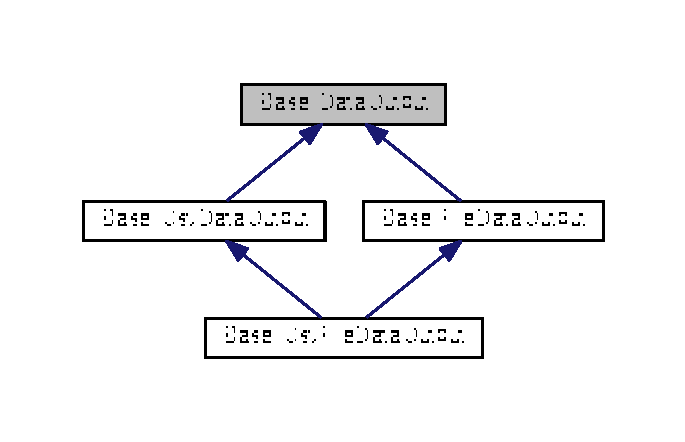
\includegraphics[width=329pt]{classBase_1_1DataOutput__inherit__graph}
\end{center}
\end{figure}
\subsection*{Public Member Functions}
\begin{DoxyCompactItemize}
\item 
virtual \hyperlink{classBase_1_1DataOutput_afbf4de9aafb25ccc5a9a1565b29565ec}{$\sim$\-Data\-Output} ()
\item 
virtual void \hyperlink{classBase_1_1DataOutput_afdb91464e7559dedf69c56c1b862a216}{Print\-Line} (int turns\-\_\-count, vector$<$ int $>$ results)=0
\item 
virtual void \hyperlink{classBase_1_1DataOutput_a0f1a6127945492d692629120575e7f82}{Print\-Column\-Titles} ()=0
\item 
virtual void \hyperlink{classBase_1_1DataOutput_a368f0c022e828cd3f29085e10e70b113}{Set\-Column\-Titles} (vector$<$ string $>$ titles)=0
\item 
virtual bool \hyperlink{classBase_1_1DataOutput_aa201a3a18e148803cc3384af60acda60}{Are\-Titles\-Printed} ()=0
\end{DoxyCompactItemize}
\subsection*{Protected Member Functions}
\begin{DoxyCompactItemize}
\item 
virtual ostream \& \hyperlink{classBase_1_1DataOutput_adea8f6af278e2e8ace25ba64d9bf9a57}{Get\-Output\-Stream} ()
\end{DoxyCompactItemize}


\subsection{Detailed Description}
Interface for printing results. Used in \hyperlink{classBase_1_1DataCollector}{Data\-Collector} for creating output of tested algorithms. 

\subsection{Constructor \& Destructor Documentation}
\hypertarget{classBase_1_1DataOutput_afbf4de9aafb25ccc5a9a1565b29565ec}{\index{Base\-::\-Data\-Output@{Base\-::\-Data\-Output}!$\sim$\-Data\-Output@{$\sim$\-Data\-Output}}
\index{$\sim$\-Data\-Output@{$\sim$\-Data\-Output}!Base::DataOutput@{Base\-::\-Data\-Output}}
\subsubsection[{$\sim$\-Data\-Output}]{\setlength{\rightskip}{0pt plus 5cm}virtual Base\-::\-Data\-Output\-::$\sim$\-Data\-Output (
\begin{DoxyParamCaption}
{}
\end{DoxyParamCaption}
)\hspace{0.3cm}{\ttfamily [inline]}, {\ttfamily [virtual]}}}\label{classBase_1_1DataOutput_afbf4de9aafb25ccc5a9a1565b29565ec}
Empty destructor 

\subsection{Member Function Documentation}
\hypertarget{classBase_1_1DataOutput_aa201a3a18e148803cc3384af60acda60}{\index{Base\-::\-Data\-Output@{Base\-::\-Data\-Output}!Are\-Titles\-Printed@{Are\-Titles\-Printed}}
\index{Are\-Titles\-Printed@{Are\-Titles\-Printed}!Base::DataOutput@{Base\-::\-Data\-Output}}
\subsubsection[{Are\-Titles\-Printed}]{\setlength{\rightskip}{0pt plus 5cm}virtual bool Base\-::\-Data\-Output\-::\-Are\-Titles\-Printed (
\begin{DoxyParamCaption}
{}
\end{DoxyParamCaption}
)\hspace{0.3cm}{\ttfamily [pure virtual]}}}\label{classBase_1_1DataOutput_aa201a3a18e148803cc3384af60acda60}
Getter for are\-\_\-titles\-\_\-printed \begin{DoxyReturn}{Returns}
True if method \hyperlink{classBase_1_1DataOutput_a0f1a6127945492d692629120575e7f82}{Print\-Column\-Titles()} was used before, false otherwise 
\end{DoxyReturn}


Implemented in \hyperlink{classBase_1_1CsvDataOutput_aaa4e604ce1d06ee002889b2604faf4e4}{Base\-::\-Csv\-Data\-Output}.

\hypertarget{classBase_1_1DataOutput_adea8f6af278e2e8ace25ba64d9bf9a57}{\index{Base\-::\-Data\-Output@{Base\-::\-Data\-Output}!Get\-Output\-Stream@{Get\-Output\-Stream}}
\index{Get\-Output\-Stream@{Get\-Output\-Stream}!Base::DataOutput@{Base\-::\-Data\-Output}}
\subsubsection[{Get\-Output\-Stream}]{\setlength{\rightskip}{0pt plus 5cm}virtual ostream\& Base\-::\-Data\-Output\-::\-Get\-Output\-Stream (
\begin{DoxyParamCaption}
{}
\end{DoxyParamCaption}
)\hspace{0.3cm}{\ttfamily [inline]}, {\ttfamily [protected]}, {\ttfamily [virtual]}}}\label{classBase_1_1DataOutput_adea8f6af278e2e8ace25ba64d9bf9a57}
Method to get stream for output. It is used only by delivery classes. \begin{DoxyReturn}{Returns}
Default stream is standard output stream 
\end{DoxyReturn}


Reimplemented in \hyperlink{classBase_1_1FileDataOutput_ae541a6775f2a1641b85e47f610618cd0}{Base\-::\-File\-Data\-Output}.

\hypertarget{classBase_1_1DataOutput_a0f1a6127945492d692629120575e7f82}{\index{Base\-::\-Data\-Output@{Base\-::\-Data\-Output}!Print\-Column\-Titles@{Print\-Column\-Titles}}
\index{Print\-Column\-Titles@{Print\-Column\-Titles}!Base::DataOutput@{Base\-::\-Data\-Output}}
\subsubsection[{Print\-Column\-Titles}]{\setlength{\rightskip}{0pt plus 5cm}virtual void Base\-::\-Data\-Output\-::\-Print\-Column\-Titles (
\begin{DoxyParamCaption}
{}
\end{DoxyParamCaption}
)\hspace{0.3cm}{\ttfamily [pure virtual]}}}\label{classBase_1_1DataOutput_a0f1a6127945492d692629120575e7f82}
Print titles of columns 

Implemented in \hyperlink{classBase_1_1CsvDataOutput_aa54484865cd138cf49b5aa5b9ef813d5}{Base\-::\-Csv\-Data\-Output}.

\hypertarget{classBase_1_1DataOutput_afdb91464e7559dedf69c56c1b862a216}{\index{Base\-::\-Data\-Output@{Base\-::\-Data\-Output}!Print\-Line@{Print\-Line}}
\index{Print\-Line@{Print\-Line}!Base::DataOutput@{Base\-::\-Data\-Output}}
\subsubsection[{Print\-Line}]{\setlength{\rightskip}{0pt plus 5cm}virtual void Base\-::\-Data\-Output\-::\-Print\-Line (
\begin{DoxyParamCaption}
\item[{int}]{turns\-\_\-count, }
\item[{vector$<$ int $>$}]{results}
\end{DoxyParamCaption}
)\hspace{0.3cm}{\ttfamily [pure virtual]}}}\label{classBase_1_1DataOutput_afdb91464e7559dedf69c56c1b862a216}
Print single line of results. 
\begin{DoxyParams}{Parameters}
{\em turns\-\_\-count} & First column of output, number of passed turns(tests) \\
\hline
{\em results} & Vector of \\
\hline
\end{DoxyParams}


Implemented in \hyperlink{classBase_1_1CsvDataOutput_a88994527237735d1d6a05cec3b222ba7}{Base\-::\-Csv\-Data\-Output}.

\hypertarget{classBase_1_1DataOutput_a368f0c022e828cd3f29085e10e70b113}{\index{Base\-::\-Data\-Output@{Base\-::\-Data\-Output}!Set\-Column\-Titles@{Set\-Column\-Titles}}
\index{Set\-Column\-Titles@{Set\-Column\-Titles}!Base::DataOutput@{Base\-::\-Data\-Output}}
\subsubsection[{Set\-Column\-Titles}]{\setlength{\rightskip}{0pt plus 5cm}virtual void Base\-::\-Data\-Output\-::\-Set\-Column\-Titles (
\begin{DoxyParamCaption}
\item[{vector$<$ string $>$}]{titles}
\end{DoxyParamCaption}
)\hspace{0.3cm}{\ttfamily [pure virtual]}}}\label{classBase_1_1DataOutput_a368f0c022e828cd3f29085e10e70b113}
Setter for titles\-\_\-names\-\_\- 
\begin{DoxyParams}{Parameters}
{\em titles} & Titles which replaces titles\-\_\-names\-\_\- \\
\hline
\end{DoxyParams}


Implemented in \hyperlink{classBase_1_1CsvDataOutput_a9302a89524b164d440280bc1c90c90d3}{Base\-::\-Csv\-Data\-Output}.



The documentation for this class was generated from the following file\-:\begin{DoxyCompactItemize}
\item 
data\-\_\-managment/data\-\_\-output.\-h\end{DoxyCompactItemize}

\hypertarget{classBase_1_1DataOutputBuilder}{\section{Base\-:\-:Data\-Output\-Builder Class Reference}
\label{classBase_1_1DataOutputBuilder}\index{Base\-::\-Data\-Output\-Builder@{Base\-::\-Data\-Output\-Builder}}
}


{\ttfamily \#include $<$data\-\_\-output\-\_\-builder.\-h$>$}



\subsection{Detailed Description}
Class generating \hyperlink{classBase_1_1DataOutput}{Data\-Output} instances using Build pattern. 

The documentation for this class was generated from the following files\-:\begin{DoxyCompactItemize}
\item 
data\-\_\-managment/data\-\_\-output\-\_\-builder.\-h\item 
data\-\_\-managment/data\-\_\-output\-\_\-builder.\-cpp\end{DoxyCompactItemize}

\hypertarget{classBase_1_1DataProvider}{\section{Base\-:\-:Data\-Provider Class Reference}
\label{classBase_1_1DataProvider}\index{Base\-::\-Data\-Provider@{Base\-::\-Data\-Provider}}
}


{\ttfamily \#include $<$data\-\_\-provider.\-h$>$}



Inherited by Base\-::\-File\-Data\-Provider.



\subsection{Detailed Description}
Interface for data providers. Data provider should return single line of input containing all elements \-:
\begin{DoxyItemize}
\item type of interaction
\item timestamp
\item sender id
\item receiver id
\end{DoxyItemize}

It is important to give access to single line multiple times (for multiple objects) 

The documentation for this class was generated from the following file\-:\begin{DoxyCompactItemize}
\item 
data\-\_\-managment/data\-\_\-provider.\-h\end{DoxyCompactItemize}

\hypertarget{classBase_1_1FileDataOutput}{\section{Base\-:\-:File\-Data\-Output Class Reference}
\label{classBase_1_1FileDataOutput}\index{Base\-::\-File\-Data\-Output@{Base\-::\-File\-Data\-Output}}
}


{\ttfamily \#include $<$file\-\_\-data\-\_\-output.\-h$>$}



Inheritance diagram for Base\-:\-:File\-Data\-Output\-:\nopagebreak
\begin{figure}[H]
\begin{center}
\leavevmode
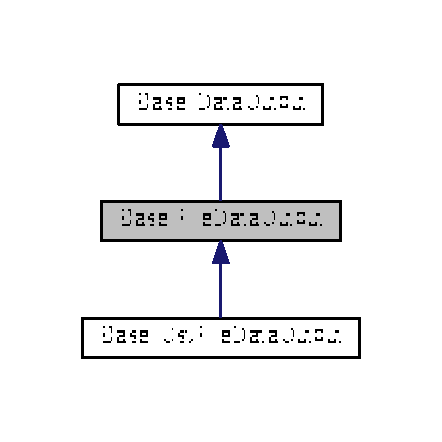
\includegraphics[width=212pt]{classBase_1_1FileDataOutput__inherit__graph}
\end{center}
\end{figure}


Collaboration diagram for Base\-:\-:File\-Data\-Output\-:\nopagebreak
\begin{figure}[H]
\begin{center}
\leavevmode
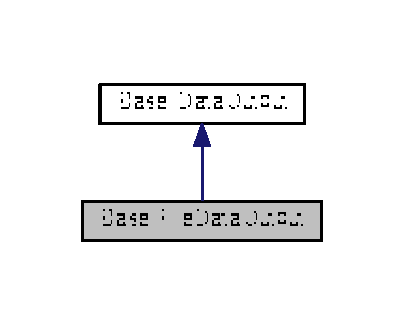
\includegraphics[width=194pt]{classBase_1_1FileDataOutput__coll__graph}
\end{center}
\end{figure}
\subsection*{Protected Member Functions}
\begin{DoxyCompactItemize}
\item 
virtual ostream \& \hyperlink{classBase_1_1FileDataOutput_ae541a6775f2a1641b85e47f610618cd0}{Get\-Output\-Stream} ()
\end{DoxyCompactItemize}
\subsection*{Additional Inherited Members}


\subsection{Detailed Description}
Role of this class is to provide output stream which write to file and take care of it. 

\subsection{Member Function Documentation}
\hypertarget{classBase_1_1FileDataOutput_ae541a6775f2a1641b85e47f610618cd0}{\index{Base\-::\-File\-Data\-Output@{Base\-::\-File\-Data\-Output}!Get\-Output\-Stream@{Get\-Output\-Stream}}
\index{Get\-Output\-Stream@{Get\-Output\-Stream}!Base::FileDataOutput@{Base\-::\-File\-Data\-Output}}
\subsubsection[{Get\-Output\-Stream}]{\setlength{\rightskip}{0pt plus 5cm}ostream \& Base\-::\-File\-Data\-Output\-::\-Get\-Output\-Stream (
\begin{DoxyParamCaption}
{}
\end{DoxyParamCaption}
)\hspace{0.3cm}{\ttfamily [protected]}, {\ttfamily [virtual]}}}\label{classBase_1_1FileDataOutput_ae541a6775f2a1641b85e47f610618cd0}
Method to get stream for output. It is used only by delivery classes. \begin{DoxyReturn}{Returns}
Default stream is standard output stream 
\end{DoxyReturn}


Reimplemented from \hyperlink{classBase_1_1DataOutput_adea8f6af278e2e8ace25ba64d9bf9a57}{Base\-::\-Data\-Output}.



The documentation for this class was generated from the following files\-:\begin{DoxyCompactItemize}
\item 
data\-\_\-managment/file\-\_\-data\-\_\-output.\-h\item 
data\-\_\-managment/file\-\_\-data\-\_\-output.\-cpp\end{DoxyCompactItemize}

\hypertarget{classMatrix_1_1MatrixBuilder}{\section{Matrix\-:\-:Matrix\-Builder Class Reference}
\label{classMatrix_1_1MatrixBuilder}\index{Matrix\-::\-Matrix\-Builder@{Matrix\-::\-Matrix\-Builder}}
}


{\ttfamily \#include $<$matrix\-\_\-builder.\-h$>$}



\subsection{Detailed Description}
Class to build \hyperlink{classMatrix_1_1MTFMatrix}{M\-T\-F\-Matrix} with appropriate parameters. 

The documentation for this class was generated from the following files\-:\begin{DoxyCompactItemize}
\item 
matrix/matrix\-\_\-builder.\-h\item 
matrix/matrix\-\_\-builder.\-cpp\end{DoxyCompactItemize}

\hypertarget{classMatrix_1_1MTFMatrix}{\section{Matrix\-:\-:M\-T\-F\-Matrix Class Reference}
\label{classMatrix_1_1MTFMatrix}\index{Matrix\-::\-M\-T\-F\-Matrix@{Matrix\-::\-M\-T\-F\-Matrix}}
}


{\ttfamily \#include $<$mtf\-\_\-matrix.\-h$>$}



\subsection{Detailed Description}
Class contains nodes in matrix with constant size rows. 

The documentation for this class was generated from the following files\-:\begin{DoxyCompactItemize}
\item 
matrix/mtf\-\_\-matrix.\-h\item 
matrix/mtf\-\_\-matrix.\-cpp\end{DoxyCompactItemize}

\hypertarget{classTools_1_1Processor}{\section{Tools\-:\-:Processor Class Reference}
\label{classTools_1_1Processor}\index{Tools\-::\-Processor@{Tools\-::\-Processor}}
}


{\ttfamily \#include $<$processor.\-h$>$}



Inheritance diagram for Tools\-:\-:Processor\-:\nopagebreak
\begin{figure}[H]
\begin{center}
\leavevmode
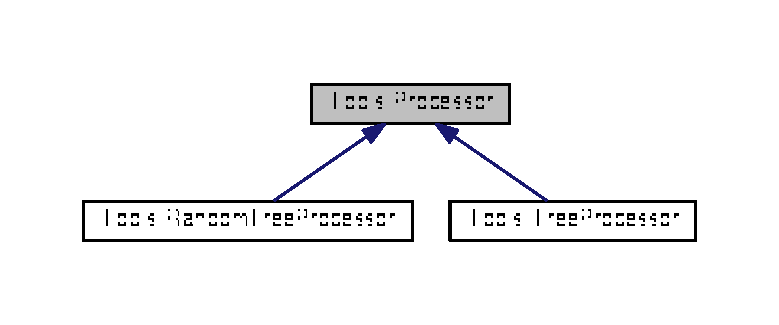
\includegraphics[width=350pt]{classTools_1_1Processor__inherit__graph}
\end{center}
\end{figure}


\subsection{Detailed Description}
Class which runs notifications of actions for one user. Subclasses can use different algorithms and penalty counters 

The documentation for this class was generated from the following files\-:\begin{DoxyCompactItemize}
\item 
tools/processor.\-h\item 
tools/processor.\-cpp\end{DoxyCompactItemize}

\hypertarget{classTools_1_1ProcessorFactory}{\section{Tools\-:\-:Processor\-Factory Class Reference}
\label{classTools_1_1ProcessorFactory}\index{Tools\-::\-Processor\-Factory@{Tools\-::\-Processor\-Factory}}
}


{\ttfamily \#include $<$processor\-\_\-factory.\-h$>$}



Inherited by Tools\-::\-Matrix\-M\-T\-F\-Processor\-Factory, Tools\-::\-M\-T\-F\-Processor\-Factory, Tools\-::\-Random\-Tree\-Processor\-Factory, and Tools\-::\-Tree\-Processor\-Factory.



\subsection{Detailed Description}
Interface to create Processors independently. It provides prepared processors for Data\-Collectors 

The documentation for this class was generated from the following file\-:\begin{DoxyCompactItemize}
\item 
tools/processor\-\_\-factory.\-h\end{DoxyCompactItemize}

\hypertarget{classTools_1_1RandomTreeProcessor}{\section{Tools\-:\-:Random\-Tree\-Processor Class Reference}
\label{classTools_1_1RandomTreeProcessor}\index{Tools\-::\-Random\-Tree\-Processor@{Tools\-::\-Random\-Tree\-Processor}}
}


{\ttfamily \#include $<$random\-\_\-tree\-\_\-processor.\-h$>$}



Inheritance diagram for Tools\-:\-:Random\-Tree\-Processor\-:\nopagebreak
\begin{figure}[H]
\begin{center}
\leavevmode
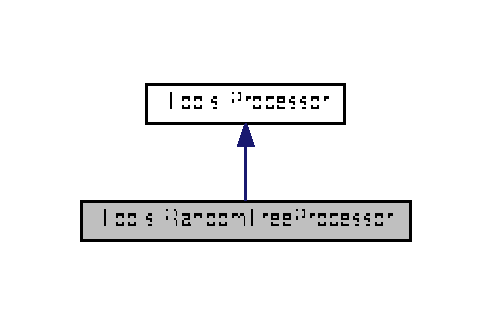
\includegraphics[width=236pt]{classTools_1_1RandomTreeProcessor__inherit__graph}
\end{center}
\end{figure}


Collaboration diagram for Tools\-:\-:Random\-Tree\-Processor\-:\nopagebreak
\begin{figure}[H]
\begin{center}
\leavevmode
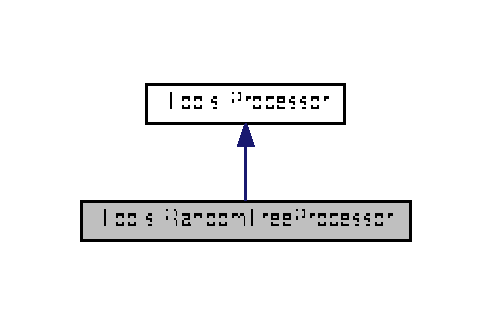
\includegraphics[width=236pt]{classTools_1_1RandomTreeProcessor__coll__graph}
\end{center}
\end{figure}


\subsection{Detailed Description}
It is processor similar to \hyperlink{classTools_1_1TreeProcessor}{Tree\-Processor}. The difference is to add random decisions how high element is push in tree during notification. 

The documentation for this class was generated from the following files\-:\begin{DoxyCompactItemize}
\item 
tools/random\-\_\-tree\-\_\-processor.\-h\item 
tools/random\-\_\-tree\-\_\-processor.\-cpp\end{DoxyCompactItemize}

\hypertarget{classTree_1_1RandomTreeRoot}{\section{Tree\-:\-:Random\-Tree\-Root Class Reference}
\label{classTree_1_1RandomTreeRoot}\index{Tree\-::\-Random\-Tree\-Root@{Tree\-::\-Random\-Tree\-Root}}
}


{\ttfamily \#include $<$random\-\_\-tree\-\_\-root.\-h$>$}



Inherits Tree\-::\-Tree\-Root.



\subsection{Detailed Description}
Class very similar to Tree\-Root. Only difference is Move\-Element method. It uses random factor influenced by different between elements to swap during moving element up.

Base algorithm is the same. If there is notification of element, algorithm tries to put it to top. During way up there is competition with elements to swap. If element looses, its parent tries to go up. 

The documentation for this class was generated from the following files\-:\begin{DoxyCompactItemize}
\item 
tree/random\-\_\-tree\-\_\-root.\-h\item 
tree/random\-\_\-tree\-\_\-root.\-cpp\end{DoxyCompactItemize}

\hypertarget{classTools_1_1Tester}{\section{Tools\-:\-:Tester Class Reference}
\label{classTools_1_1Tester}\index{Tools\-::\-Tester@{Tools\-::\-Tester}}
}


{\ttfamily \#include $<$tester.\-h$>$}



\subsection{Detailed Description}
Class counts penalty 

The documentation for this class was generated from the following files\-:\begin{DoxyCompactItemize}
\item 
tools/tester.\-h\item 
tools/tester.\-cpp\end{DoxyCompactItemize}

\hypertarget{classTools_1_1TreeProcessor}{\section{Tools\-:\-:Tree\-Processor Class Reference}
\label{classTools_1_1TreeProcessor}\index{Tools\-::\-Tree\-Processor@{Tools\-::\-Tree\-Processor}}
}


{\ttfamily \#include $<$tree\-\_\-proccessor.\-h$>$}



Inheritance diagram for Tools\-:\-:Tree\-Processor\-:\nopagebreak
\begin{figure}[H]
\begin{center}
\leavevmode
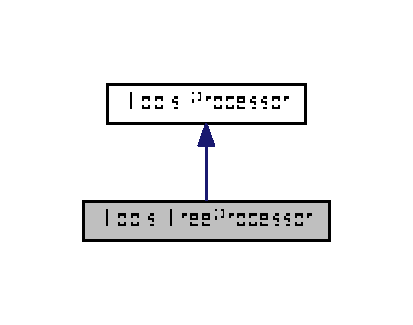
\includegraphics[width=198pt]{classTools_1_1TreeProcessor__inherit__graph}
\end{center}
\end{figure}


Collaboration diagram for Tools\-:\-:Tree\-Processor\-:\nopagebreak
\begin{figure}[H]
\begin{center}
\leavevmode
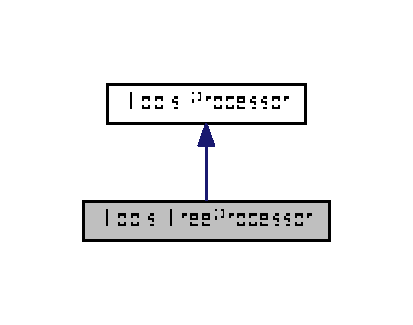
\includegraphics[width=198pt]{classTools_1_1TreeProcessor__coll__graph}
\end{center}
\end{figure}


\subsection{Detailed Description}
\hyperlink{classTools_1_1Processor}{Processor} based on tree structure. It works like Move To Front, but Move To Top Of Tree is the best words to describe how it works.

It uses Tree\-Root as data structure with Tree\-Factory to generate new elements 

The documentation for this class was generated from the following files\-:\begin{DoxyCompactItemize}
\item 
tools/tree\-\_\-proccessor.\-h\item 
tools/tree\-\_\-proccessor.\-cpp\end{DoxyCompactItemize}

%--- End generated contents ---

% Index
\newpage
\phantomsection
\addcontentsline{toc}{chapter}{Index}
\printindex

\end{document}
